\documentclass[11pt, oneside]{article} 
\usepackage{geometry}
\geometry{letterpaper} 
\usepackage{graphicx}
	
\usepackage{amssymb}
\usepackage{amsmath}
\usepackage{parskip}
\usepackage{color}
\usepackage{hyperref}

\graphicspath{{/Users/telliott_admin/Tex/png/}}
% \begin{center} 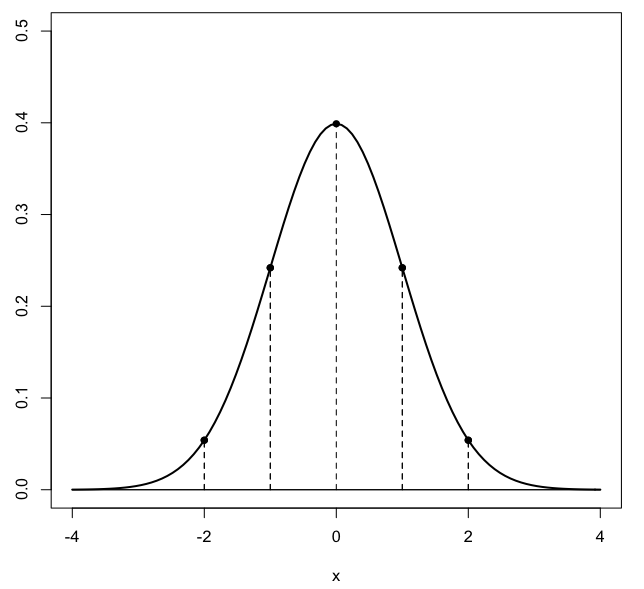
\includegraphics [scale=0.4] {gauss3.png} \end{center}

\title{Sum of angles, Euler}
\date{}

\begin{document}
\maketitle
\Large

\label{sec:Euler_sum_angles}

Euler's equation says that
\[ e^{i\theta} = \cos \theta + i \sin \theta \]

One way of thinking about the equation is to view complex numbers as points in the plane.  Complex numbers are composed of a real part (say $x$) and a complex part $(iy)$, where $i = \sqrt{-1}$.

\begin{center} 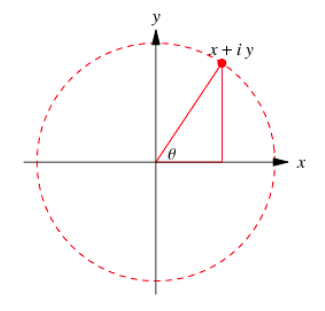
\includegraphics [scale=0.5] {argand.png} \end{center}

It turns out that $e^{i\theta}$ corresponds to the specification of such a point in radial coordinates in the \emph{Argand} or complex plane.

Later, we will look at a quick derivation of Euler's equation.

One valid proof is to simply plug into the series for the exponential
\[ e^x = 1 + x + \frac{x^2}{2!} + \frac{x^3}{3!} + \frac{x^4}{4!} + \frac{x^5}{5!} + \dots \]
giving
\[ e^{ix} = 1 + ix - \frac{x^2}{2!} - i \frac{x^3}{3!} + \frac{x^4}{4!} + i \frac{x^5}{5!} + \dots \]
\[ = \cos x + i \sin x \]

which, I realize, we also haven't seen yet.   So, take it on faith for the moment.

We can use Euler's equation to get something extremely useful for calculus.

\subsection*{using Euler}

Switch notation to $s$ and $t$
\[ e^{i s} = \cos s + i \sin s \]
\[ e^{i t} = \cos t + i \sin t \]
\[ e^{i (s+t)} = \cos (s+t) + i \sin (s+t) \]

But
\[ e^{i (s+t)} = e^{i s} e^{i t} \]
\[ = (\cos s + i \sin s) \ (\cos t + i \sin t) \]
\[ = \cos s \cos t + \cos s \ i \sin t + i \sin s \cos t - \sin s \sin t \]
\[ = (\cos s \cos t - \sin s \sin t) + i (\sin s \cos t + \cos s \sin t ) \]

We have an equality between two complex numbers, both equal to $e^{i (s+t)}$.  For this to be true, both the real and imaginary parts must be equal.

\[ \cos (s+t) = \cos s \cos t - \sin s \sin t \]
\[ \sin (s+t) = \sin s \cos t + \cos s \sin t \]

The addition formulas for sine and cosine.  

I find that this is an extremely useful way of remembering how these formulas can be derived.


\end{document}  